\documentclass[
    reprint,
    superscriptaddress,
    a4paper,
    amsmath,amssymb,
    prl,
]{revtex4-2}
\usepackage{graphicx, color} %


\usepackage[dvipsnames]{xcolor}
\definecolor{APSBlue}{HTML}{2e3092}
\usepackage[
    colorlinks,
    citecolor=APSBlue,
    linkcolor=APSBlue,
    urlcolor=APSBlue,
]{hyperref}
\usepackage{lipsum}
\usepackage{comment}

\usepackage{textcomp}
\usepackage{graphicx}
\usepackage{fixmath}
\usepackage{xcolor}


\usepackage{stackengine}
\setstackgap{S}{1pt}

\newcommand{\boldsf}[1]{\textsf{\textbf{#1}}}

\usepackage{physics}

\newcommand{\qqoute}[1]{``#1''}
\newcommand{\const}{\operatorname{const}}

\newcommand{\iu}{\mathrm{i}\mkern1mu}
\newcommand{\eu}{\mathrm{e}\mkern1mu}

\newcommand{\red}[1]{\textcolor{red}{#1}}
\newcommand{\blue}[1]{\textcolor{blue}{#1}}
\newcommand{\green}[1]{\textcolor{Green}{#1}}
\newcommand{\gray}[1]{\textcolor{gray}{#1}}

\newcommand{\Refs}{\textbf{\red{[Refs]}}}
\newcommand{\RefsWho}[1]{\textbf{\red{[#1]}}}

\usepackage{xspace}  
\usepackage{chemformula}
\newcommand{\VOtwo}{VO\textsubscript{2}\xspace}
\newcommand{\VOtwox}{VO\(_{2-x}\)\xspace}

\newcommand{\VtwoOfive}{V\textsubscript{2}O\textsubscript{5}\xspace}
\newcommand{\celsius}{\textcelsius\xspace}

\newcommand{\SiOtwo}{SiO\textsubscript{2}\xspace}
\newcommand{\SM}{Supplementary Material\xspace}

\newcommand{\IT}[1]{\red{\textbf{Ivan Toftul}: #1.\xspace}}

\newcommand{\KK}[1]{\blue{#1\xspace}}

\newcommand{\PT}[1]{\green{\textbf{Pavel}: #1.\xspace}}

\newcommand{\affilANU}{Nonlinear Physics Center, Research School of Physics, Australian National University, Canberra ACT 2601, Australia}

\newcommand{\affilHarbin}{Ministry of Industry and Information Technology Key Lab of Micro-Nano Optoelectronic Information System, Guangdong Provincial Key Laboratory of Semiconductor
Optoelectronic Materials and Intelligent Photonic Systems, Harbin Institute of Technology, Shenzhen 518055, P.R. China}

\newcommand{\affilMoscow}{ Shubnikov Institute of Crystallography, NRC “Kurchatov Institute”, Moscow 119333, Russia}



\begin{document}

\title{Chiral dichroism in resonant metasurfaces with monoclinic lattices}

\author{Ivan Toftul}
\email{ivan.toftul@anu.edu.au}
\affiliation{\affilANU}

\author{Pavel Tonkaev}
\affiliation{\affilANU}

\author{Kirill Koshelev}
\affiliation{\affilANU}

\author{Fangxing Lai}
\affiliation{\affilHarbin}


\author{Qinghai Song}
\affiliation{\affilHarbin}

\author{Maxim Gorkunov}
\affiliation{\affilMoscow}

\author{Yuri Kivshar}
\email{yuri.kivshar@anu.edu.au}
\affiliation{\affilANU}


\begin{abstract}
 We reveal that chiral response can be achieved in resonant metasurfaces with a monoclinic lattice symmetry (the so-called Bravais {\it oblique lattices}) where the mirror symmetry is broken by the lattice asymmetry and by a substrate, while each individual meta-atom remains fully {\it achiral}. We describe the underlying mechanism
 by introducing the mode chirality parameter as a quantitative measure of the lattice chiral eigenmodes. We confirm experimentally selective linear and nonlinear chiral interaction of resonant silicon metasurfaces with circularly polarized light.
\end{abstract}

\maketitle



\textit{Introduction.}---Traditionally, chiral response of a metasurface is achieved by engineering the \textit{shape} of meta-atoms. It is done by shaping metallic meta-atoms~\cite{Papakostas2003Mar,Ren2012May} or by creating multilayer~\cite{Tanaka2020Nov} or single layer asymmetric dielectric structures~\cite{Koshelev2023ACSPhot}.
Another option is to utilize the \textit{rotation} of meta-atoms with respect to the overall metasurface lattice.
The later possibility was discussed theoretically~\cite{Movsesyan2022Jul,Avalos-Ovando2022Jul} and demonstrated  experimentally~\cite{Gryb2023Oct} very recently.
However, these methods generally require meta-atoms with inherent non-continuous rotational symmetry (i.e., lacking infinite rotational symmetry, $C_{\infty}$).

\begin{figure*}
    \centering
    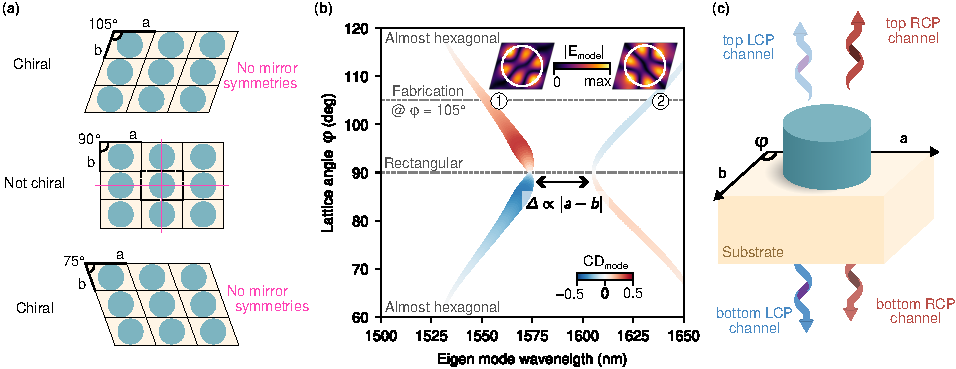
\includegraphics[width=1\linewidth]{fig1_concept_and_CDm_v4.pdf}
    \caption{
    \textbf{The concept of chiral metasurfaces build of achiral meta-atoms}. 
    \textbf{(a)} Absence of mirror symmetry planes makes the metasurface geometrically chiral. One of the possible ways is to use monoclinic lattice arrangement of simple-shaped achiral meta-atoms, such as cylinders.
    \textbf{(b)} Metasurface eigenmodes acquire chirality once the lattice angle is not equal to $90^{\circ}$, i.e., the lattice is not rectangular.
    To avoid mode degeneracy at $\varphi = 90^{\circ}$, the lattice constants are taken unequal, $a\neq b$, and we observe a typical anti-crossing behaviour. 
    At the angles of $\varphi = 60^{\circ}$ and $120^{\circ}$ the lattice becomes very close to hexagonal and the mode chirality vanishes as this lattice has the highest number of in-plane mirror symmetry planes.
    \textbf{(c)} Schematic of a chiral mode differently coupled with RCP and LCP channels. 
    }
    \label{fig:concept}
\end{figure*}

While extrinsic chirality manifested for obliquely incident beams is a well-established phenomenon~\cite{Plum2009May,Asefa2023Sep}, it often necessitates complex setups and may not be ideal for practical applications. 
Here we propose how to %
achieve both linear and nonlinear intrinsic chiral optical responses at \textit{normal} incidence utilizing ultimately symmetric achiral cylindrical meta-atoms arranged in monoclinic (in terms of 2D Bravais lattice types) lattices. 
The approach opens a broad avenue for manipulating chiral light-matter interactions, and it will substantially facilitate many useful practical applications due to the ultimate simplicity of required metastructures.



\begingroup
\squeezetable
\begin{table}
\caption{\label{tab:summary}Summary of metasurface chiral 
transmission characteristics, approximations at the resonance in the pump frequency range, and symmetry requirements.}
\begin{ruledtabular}
\begin{tabular}{lccc}
Characteristics                                                     & Definitions & \begin{tabular}[c]{@{}c@{}} Res. approx.\\ $\omega \approx \omega^{\prime}_n$\end{tabular}   & $\neq 0$ if  \\ \hline
\begin{tabular}[c]{@{}l@{}}Linear CD \\ (side independent)\end{tabular}                                                        &   Eq.~\eqref{eq:CDco}         &     Eq.~\eqref{eq:CDmode}                          & \begin{tabular}[c]{@{}c@{}}true chiral \\ (no mirror sym.)\end{tabular} \vspace{0.4cm} \\
\begin{tabular}[c]{@{}l@{}}Nonlinear CD \\ (pump from air)\end{tabular} &      Eq.~\eqref{eq:NCDtot}       &   Eq~\eqref{eq:NCDn}   &   no in-plane sym.                        \vspace{0.4cm} \\
\begin{tabular}[c]{@{}l@{}}Nonlinear CD \\ (pump from subs.)\end{tabular} &       \begin{tabular}[c]{@{}c@{}}Eq~\eqref{eq:NCDtot} \\ ($I^{(3\omega)} \to I^{\prime (3\omega)}$)\end{tabular}     &    \begin{tabular}[c]{@{}c@{}}Eq~\eqref{eq:NCDn} \\ ($m \to m^{\prime}$)\end{tabular}   &      no in-plane sym.
\end{tabular}
\end{ruledtabular}
\end{table}
\endgroup

\textit{Concept and theoretical prediction.}---Chirality is a geometric property according to which an object is mirror-asymmetric, or, equivalently, different from its image seen in a mirror, irrespective of orientation~\cite{Caloz2020Feb}.
The metasurface made of rotationally symmetric meta-atoms distributed in a monoclinic lattice on a substrate is chiral, Fig.~\ref{fig:concept}{(a)}.
This mirror asymmetry can be optically detected by exposing the object of interest to right circularly polarized (RCP) light and left circularly polarized (LCP) light.
The conventional characteristic is \textit{circular dichroism} (CD) which is originally defined as a difference in \textit{absorption} of RCP and LCP light, and this definition is widely adopted in chemistry and biology~\cite{fasman2013circular,Kobayashi2011Nov,Baase1979Feb}. 
In the context of dielectric metasurfaces, the CD definition becomes less related to absorption, as drastically different response to LCP and RCP light is possible in lossless structures~\cite{Hu2017Jan,Gorkunov2020Aug,Kim2020Aug}.
Moreover, in metasurfaces of different point symmetry, the asymmetry of right-to-right and left-to-left \textit{co-polarized transmission} can be accompanied by the right-to-left  and left-to-right \textit{cross-polarized transmission} 
asymmetry \cite{Koshelev2024JOPT}. 
As, nevertheless, a reciprocal achiral structure must have symmetric co-polarized  transmission, the co-polarized CD defined as
\begin{equation}
    \mathrm{CD}_{\text{co}} = \frac{\abs{t_{\text{RR}}}^2 - \abs{t_{\text{LL}}}^2}{\abs{t_{\text{RR}}}^2 + \abs{t_{\text{LL}}}^2} = \frac{\abs{t^{\prime}_{\text{RR}}}^2 - \abs{t^{\prime}_{\text{LL}}}^2}{\abs{t^{\prime}_{\text{RR}}}^2 + \abs{t^{\prime}_{\text{LL}}}^2}
    \label{eq:CDco}
\end{equation}
remains an explicit characteristic of the geometric chirality. 
It varies between $-1$ and $+1$, and here $t_{\text{RR}}$ and $t_{\text{LL}}$ are the complex transmission coefficients in the circular basis, with the first and last indexes denoting the output and input polarizations, correspondingly; primed transmission coefficients describe the case of excitation from the opposite side, i.e., from a substrate.
$\mathrm{CD}_{\text{co}}$ in Eq.~\eqref{eq:CDco} is independent of the input direction as long the structure consists of electromagnetically reciprocal materials. 
The Lorentz reciprocity imposes different limitations on the reflection coefficients, as it requires the equality $r_{RL}=r_{LR}$ at the normal incidence, regardless of the metasurface symmetry~\cite{Koshelev2024JOPT,Gorkunov2024}. 
The summary of metasurface chiral transmission characteristics studied in this Letter is in Tab.~\ref{tab:summary}.


While a mirror asymmetric metasurface is allowed to have $\mathrm{CD}_{\text{co}} \neq 0$, symmetry breaking does not guarantee that CD reaches high values. This requires careful engineering of metasurface structure, which, in particular, determines the spatial structure of metasurface photonic eigenmodes. 
Particularly attractive are high quality factor (high-$Q$) modes selectively coupled to an RCP or an LCP radiation channel. Chiral bound states in the continuum are representative examples of such modes~\cite{Gorkunov2020Aug,Overvig2021Feb,kuhner2023}.

In this Letter, we adopt and develop a highly efficient predictive method which allows designing strongly chiral metasurfaces based only on the fast eigenmodes calculations rather than on computationally expensive full numeric transmission calculations.
We assume that in the vicinity of the resonance, the metasurface response is determined by a single resonant mode. By applying the coupled mode theory, we can quantify the eigenmode contribution to the chiral optical properties, and hence the potential values of $\mathrm{CD}_{\text{co}}$. It is particularly useful to introduce the \textit{mode circular dichroism}, $\mathrm{CD}_{\text{mode},n}$, as~\cite{SM}
\begin{equation}
    \mathrm{CD}_{\text{mode},n} = \frac{\abs{m^{\prime}_{n \text{R}}m_{n\text{R}}}^2 - \abs{m^{\prime}_{n\text{L}}m_{n\text{L}}}^2}{\abs{m^{\prime}_{n\text{R}}m_{n\text{R}}}^2 + \abs{m^{\prime}_{n\text{L}}m_{n\text{L}}}^2}
    \label{eq:CDmode}
\end{equation}
where the parameters of the mode coupling to RCP and LCP waves are introduced as~\cite{Weiss2018PRB,Gorkunov2020Aug,koshelev2022PhDthesis,Koshelev2020Science}:
\begin{equation}
    m_{n\text{R,L}} = A_n \int \limits_{\text{meta}} \Delta \varepsilon (\vb{r}) \vb{E}_n (\omega_n, \vb{r}) \cdot \vb{E}_{\text{bg}}^{(\mathrm{R}, \mathrm{L})} (\omega_n, \vb{r}) \dd^{3} \vb{r}
    \label{eq:m}
\end{equation}
with the eigenmode electric field $\vb{E}_n$ and the background electric field of RCP or LCP wave $\vb{E}_{\text{bg}}^{(\mathrm{R},\mathrm{L})}$ including the Fresnel fields reflected and transmitted by the substrate without the metasurface~\cite[Sec.~VI]{Weiss2018PRB}. 
$\Delta \varepsilon (\vb{r})$ denotes the difference between the permittivities of the metasurface and the background which in our case includes the substrate.
The primed coupling parameters in \eqref{eq:CDmode} describe the coupling to the waves incident on the back metasurface side. See also Fig.~\ref{fig:concept}{(c)} for the illustration of the outgoing channels.
The $A_n$ is the normalization coefficient. A symmetric magnetic counterpart of Eq.~\eqref{eq:m} is absent due to the non-magnetic nature of the materials, i.e., $\Delta \mu (\vb{r}) =0$.


Coefficient $A_n$ is unique for each mode, which includes the eigenmode normalization, perturbation of the permittivity, and other constants~\cite[see Appendix]{koshelev2022PhDthesis} but we don't provide its explicit form as it cancels out in Eq.~\eqref{eq:CDmode}.


\begin{figure*}
    \centering
    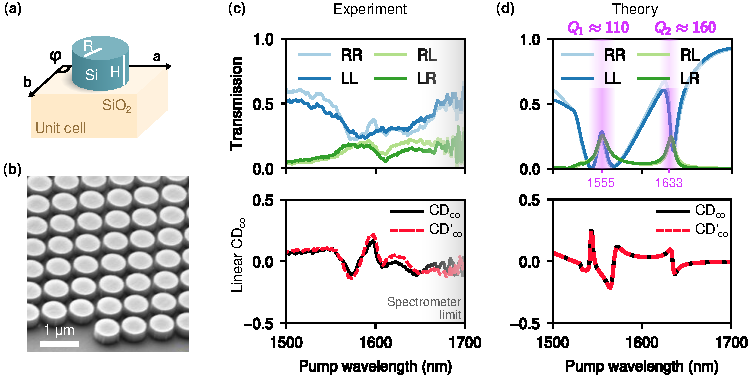
\includegraphics[width=0.85\linewidth]{fig2_linear_spectra_v4.pdf}
    \caption{
    \textbf{Linear optical properties}. 
    \textbf{(a)} Schematic representation of the metasurface unit cell with all geometrical parameters.
    \textbf{(b)} Scanning electron microscope image of a fragment of fabricated sample.
    \textbf{(c)} and \textbf{(d)} are the experimental and theoretical spectra of linear transmission coefficients and circular dichroism.
    Theory predict the position of two modes at $\lambda_{1}^{\text{res}} = 1555$~nm and at $\lambda_{2}^{\text{res}} = 1633$~nm with quality factors of $Q_1 \approx 110$ and $Q_2 \approx 160$, respectively. $\mathrm{CD}_{\text{co}}$ and $\mathrm{CD}^{\prime}_{\text{co}}$ denote co-polarized CD of transmission of light incident from the air and from the substrate correspondingly.   
    }
    \label{fig:linear}
\end{figure*}

We start our design with the Si cylinders in a rectangular lattice ($a\neq b$, $\varphi = 90^{\circ}$, Fig.~\ref{fig:concept}{(a)}) placed on a substrate made of SiO$_2$. 
The two eigenmodes of interest, which electric field distribution is shown in the inset of Fig.~\ref{fig:concept}{(b)}, are coupled to each other. The degeneracy is removed by making the lattice rectangular rather than square, i.e. spectral distance between the eigenmodes increases as $\Delta \propto |a - b|$, where $a$ and $b$ stand for the lattice spacings~\cite{SM}. The out-of-plane mirror symmetry is {\it intrinsically broken} by the substrate. Next, we break all in-plane mirror symmetries by making the lattice monoclinic. The optimal monoclinic lattice angle, $\varphi$, can be obtained by examining Fig.~\ref{fig:concept}{(b)}, where we plot the mode circular dichroism~\eqref{eq:CDmode} for these modes.
As expected, for $\varphi = 90^{\circ}$, the mode circular dichroism is zero, $\mathrm{CD}_{\text{mode}} = 0$, as the lattice is rectangular and has 2 in-plane mirror symmetries. For lattice angles $\varphi = 60^{\circ}$ or $\varphi = 120^{\circ}$ we obtain $\mathrm{CD}_{\text{mode}} \approx 0$ as the metasurface lattice approaches a hexagonal lattice, which has 6 in-plane mirror symmetries.
For intermediate $\varphi$ values, there are no mirror symmetries which results in non-zero mode chirality parameter values, $\mathrm{CD}_{\text{mode}} \neq 0$. 
Metasurfaces with $\varphi = 90^{\circ} - \Delta \varphi$   and $\varphi = 90^{\circ} + \Delta \varphi$ are enantiomers, where $\Delta \varphi$ ranges from $0^{\circ}$ to $30^{\circ}$.


Mode circular dichroism \eqref{eq:CDmode} is not directly related to the circular dichroism~\eqref{eq:CDco}, and  $\mathrm{CD}_{\text{mode}} \approx \mathrm{CD}_{\text{co}}\big|_{\omega = \Re(\omega_n)}$ only in the vicinity of the resonance when contribution of all other modes is negligibly small and the background achiral transmission is absent~\cite{SM}. 

\textit{Experimental realization.}---To prove our theoretical prediction we have fabricated metasurfaces, Fig.~\ref{fig:linear}(b). The design parameters were $a = 1100$~nm, $b=1000$~nm, $R = 430$~nm, $H = 400$~nm, and $\varphi = 75$~deg, Fig.~\ref{fig:linear}(a). The samples were fabricated using a combination of electron beam lithography, lift-off processes, and reactive ion etching (RIE), see~\cite{SM} for more details. 
To compare with our theoretical predictions shown in Fig.~\ref{fig:linear}{(d)} we measure the transmission of RCP and LCP near-IR light through the metasurface. The incoming and outgoing circular light polarizations are set by polarizers and quarter wave plates in front of and behind the sample. The recorded spectra including two co-polarised (LL and RR) and two cross-polarised (LR and RL) transmittances are shown in Fig.~\ref{fig:linear}{(c)}. The co-polarised spectra demonstrate peaks that shifted related to each other, Similar behaviour is observed for cross-polarised spectra. We expected the second resonant mode near 1700 nm, however, due to the low sensitivity of the spectrometer the resonant mode is non-pronounced in the recorded spectra. The calculated from the experimental data CD according to Eq.~\eqref{eq:CDco} is shown in Fig.~\ref{fig:linear}{(c)}. Overall, linear CD exhibits a value close to $0$, and changes from $-0.2$ to $+0.2$ near the resonance wavelength. 


\begin{figure}[h!]
    \centering
    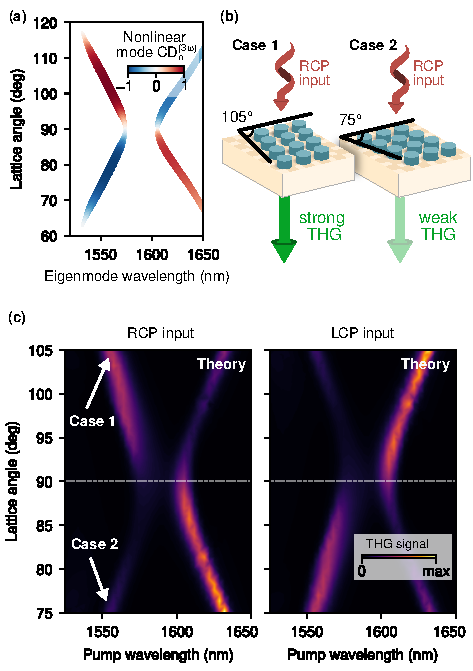
\includegraphics[width=1\linewidth]{fig3_nonlinear_theory_v5.pdf}
    \caption{\textbf{Nonlinear theory}.
    \textbf{(a)} Mode nonlinear circular dichroism calculated via coupled mode theory for the excitation from the top.
    \textbf{(b)} Example of two metasurfaces with opposite handedness (enantiomer). Once the mode of the excitation wavelength has a high chirality parameter it is coupled better with RCP input rather than LCP input or vice versa. Once the coupling strength is high for a particular input, this leads to a higher energy transfer into the THG signal.
    The chessboard pattern is a guide for the eye to show a rectangular lattice. 
    \textbf{(c)} THG signal as a function of the lattice angle and the pump wavelength. For a rectangular lattice, i.e. $\varphi = 90^{\circ}$, THG signals are identical for both input polarization. However, the change of the lattice angle below or above $90^{\circ}$ one can see that one branch is brighter for one inclination and darker for another. This directly correlates with the eigenmode analyses made in Fig.~\ref{fig:concept}.
    }
    \label{fig:nonlinear_theory}
\end{figure}


\textit{Nonlinear circular dichroism.}---While linear circular dichroism is well defined via the partial transmission, the definition of the \textit{nonlinear circular dichroism}, $\mathrm{CD}^{(n \omega)}$, is not fully settled in the literature.
The common option is to define nonlinear CD via total transmitted intensities from RCP and LCP inputs~\cite{SM,Petralli-Mallow1993JPhysChem,Kim2020NanoLett,Frizyuk2021NanoLett,Tang2020LaserPhotonicsRev}
\begin{equation}
    \mathrm{CD}^{(3\omega)} = \frac{I_{\text{R}}^{(3\omega)} - I_{\text{L}}^{(3\omega)}}{I_{\text{R}}^{(3\omega)} + I_{\text{L}}^{(3\omega)}} 
    \label{eq:NCDtot}
\end{equation}
where $I^{(3\omega)}_{\text{R(L)}}$ is the intensity of the third harmonic signal for RCP (LCP) input beam on the fundamental frequency.
Surprisingly, using nonlinear coupled mode theory it is possible to derive a very compact expression for the nonlinear $\mathrm{CD}^{(3\omega)}$ via coupling parameters given by Eq.~\eqref{eq:m} once there is a prominent resonance at the pump frequency, i.e. $\omega \approx \Re ( \omega_n)$, so \(\mathrm{CD}^{(3\omega)} \approx \mathrm{CD}^{(3\omega)}_n\), where~\cite{SM,Koshelev2023ACSPhot}
\begin{equation}
    \mathrm{CD}^{(3\omega)}_n = \frac{|m_{n\text{R}}|^6-|m_{n\text{L}}|^6}{|m_{n\text{R}}|^6+|m_{n\text{L}}|^6}.
    \label{eq:NCDn}
\end{equation}
For the excitation from the substrate one must substitute primed $m$-coupling parameters into Eq.~\eqref{eq:NCDn}. In the absence of top-down mirror symmetry, in general, $|m_{n\text{R(L)}}| \neq |m^{\prime}_{n\text{R(L)}}|$. 
Only recently the relation between the symmetry constraints and output signals in nonlinear transmission was studied~\cite{Koshelev2024JOPT}. In particular, in the presence of in-plane mirror symmetries $\mathrm{CD}^{(3\omega)}$ must be zero. For the monoclinic lattice, $\mathrm{CD}^{(3\omega)} \neq 0$ is allowed.
Remarkably, the true geometric chirality is not required for this, as even in the presence of out-of-plane mirror symmetry plane, different third harmonic signals can be generated by RCP or LCP pumping waves. {We note that this effect was previously associated with asymmetric nonlinear transmission in metallic metasurfaces~\cite{Achouri2018IEEE}, and can be predicted from the symmetry properties of full nonlinear scattering matrix}.  
In such case, however, the sign of nonlinear CD \eqref{eq:NCDtot} has to be opposite for the pumping incident on different metasurface sides~\cite{SM,Koshelev2024JOPT}.
In the case studied here, the geometric chirality is ensured by the presence of a transparent substrate. See Table~\ref{tab:summary} for the summary of the linear and nonlinear chiral characteristics.

In contrast to linear mode CD \eqref{eq:CDmode}, which is constructed from the symmetric combination of primed and non-primed coupling parameters \eqref{eq:m}, the mode nonlinear CD \eqref{eq:NCDn} is \textit{side dependent}.
Structures with out-of-plane mirror symmetry must have $\mathrm{CD}_n^{(3\omega)} = - \mathrm{CD}_n^{\prime (3\omega)}$, where prime means that one should use $m^{\prime}_{n\text{R},\text{L}}$ in Eq.~\eqref{eq:NCDtot}. For our design we have the most general case with $|\mathrm{CD}_n^{(3\omega)}| \neq |\mathrm{CD}_n^{\prime (3\omega)}|$. 


\begin{figure*}
    \centering
    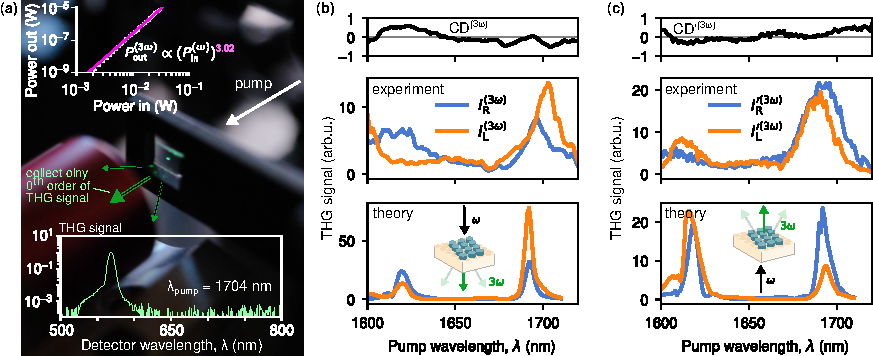
\includegraphics[width=0.98\linewidth]{fig4_nonlinear_exp_v5.pdf}
    \caption{
    \textbf{Nonlinear experiment}.
    \textbf{(a)} Photo of the experimental setup. The intensity of the THG is sufficient to observe it by the naked eye.
    Inset top: power to power dependence is well fitted by $P_{\text{out}}^{(3\omega)} \approx 0.27 (P_{\text{in}}^{(\omega)} )^{3.02}$ which is a sign that undepleted pump approximation is valid.
    Inset bottom: typical THG signal spectrum at the detector.
    \textbf{(b,c)} Total THG signal for RCP and LCP inputs and calculated nonlinear circular dichroism for excitations from the air and from the substrate. One can see a significant difference indicating that the fabricated metasurface indeed exhibits strong intrinsic nonlinear chirality. Theoretical spectra are shifted by the $+60$~nm to match the positions of peaks observed experimentally.
    }
    \label{fig:nonlinear_exp}
\end{figure*}


Since third harmonic generation is a relatively low efficient process, the resonant enhancement is crucial for any potential practical application. A resonance at the fundamental harmonic wavelength is preferable to a resonance at the third harmonic wavelength due to the potential signal enhancement by factor of $Q^3$, which is the highest possible excluding double resonant conditions requiring sophisticated designs~\cite{Koshelev2020Science}. 
The effects of the chiral resonance at the high harmonic frequency were also discussed in the literature~\cite{Antonov2023ieee_proceeding} but it is out of scope this work.
Values close to $+1$ ($-1$) of the nonlinear circular dichroism defined by Eq.~\eqref{eq:NCDtot} suggest that RCP (LCP) input is much more efficient in terms of amount of energy converted to the third harmonic domain. 

In Fig.~\ref{fig:nonlinear_theory} we vary the lattice angle in the same manner as in Fig.~\ref{fig:concept}{(b)} but now examine the third harmonic signal in transmission collecting only the $0$-th diffraction order. 
Fig.~\ref{fig:nonlinear_theory}{(a)} shows the  nonlinear mode $\mathrm{CD}^{(3\omega)}$~\eqref{eq:NCDn} for the excitation from the top, while
Fig.~\ref{fig:nonlinear_theory}{(b)} demonstrates that for a chiral mode, the coupling strength with different light polarizations becomes asymmetric for the nonlinear signal as well. 
This leads to a stronger interaction with the preferred polarization, resulting in a higher intensity of the third-harmonic generation signal. The figure visually depicts this effect for different lattice angles.
One can see a clear correspondence of the nonlinear mode CD and third harmonic signal intensities (compare panels (a) and {(c)} in Fig.~\ref{fig:nonlinear_theory}). 



We also prove this prediction experimentally. To study nonlinear properties of metasurfaces we use a tunable near-IR laser with a pulse duration of 500 fs and repetition rate of 5.14 MHz. Fig.~\ref{fig:nonlinear_exp} presents the observed THG signal pumped with a peak laser intensity of 4~GW/cm$^2$: strong enough to be visible to the naked eye. The THG spectrum exited at the resonant wavelength of 1700 nm measured in transmission is shown in Figs.~\ref{fig:nonlinear_exp}{(b,c)}. The THG spectrum has a maximum at wavelength 568 nm and linewidth of 7 nm. We also record the power dependence of THG shown in the inset of Fig.~\ref{fig:nonlinear_exp}(a). The obtained curve has a good agreement with cubic law: $P_{\text{out}}^{(3\omega)} \approx 0.27 (P_{\text{in}}^{(\omega)} )^{3.02}$ which is a sign that undepleted pump approximation is valid.


To investigate the resonant properties of THG generated from the metasurface, we pump it by a femtosecond laser with wavelengths in the range of 1500-1730 nm with a 1~nm step from two sides: from the air and from the substrate. The recorded THG spectra for RCP and LCP excitation show two distinct peaks corresponding to the two chiral modes studied above, see them compared with the theoretical THG spectra in Figs.~\ref{fig:nonlinear_exp}(b,c). In all cases, THG signals demonstrate resonant enhancement near two wavelengths corresponding to the resonant modes observed in the linear regime. Next, we evaluate the experimental nonlinear CD according to Eq.~(\ref{eq:NCDtot}) as seen on the top panels of Figs.~\ref{fig:nonlinear_exp}(b,c). Being driven by the resonances, nonlinear CD varies from $-0.64$ to $0.32$ for different pump wavelengths. 


\textit{Conclusions.---}We have proposed and verified that the monoclinic geometry of metasurface lattices leads to distinct intrinsic chiral optical response, both in the linear and nonlinear regimes, even if metasurfaces are composed of highly symmetric achiral elements. We have developed a general analytical approach to characterize such metasurfaces by the mode chirality parameter as a quantitative measure of the eigenmode contribution to linear and nonlinear optical chirality. We have demonstrated experimentally the intrinsic chiral response of monoclinic silicon metasurfaces in both linear and nonlinear regimes.



\begin{acknowledgements}
Y.K. thanks Kuniaki Konishi, Olivier Martin, and Yuri Svirko for useful discussions.  
Authors thank Shumin Xiao for valuable suggestions to the fabrication.
This work was supported by the Australian Research Council (Grant No. DP210101292), the International Technology Center Indo-Pacific (ITC IPAC) via Army Research Office (contract FA520923C0023), National Natural Science Foundation of China (Grants 12261131500 and 12025402), and Shenzhen Fundamental Research Projects (grant JCYJ20210324120402006). M.G. acknowledges a support from the Russian Science Foundation (Project 23-42-00091).
\end{acknowledgements}




 


\bibliography{refs}

\end{document}
